An important part of this work is a toolchain embodying the methodology. The
toolchain has been implemented in the Rust programming language
\cite{rust}.\footnote{Rust is a systems programming language developed by
Mozilla Research and thousands of independent contributors from all around the
world. Rust provides memory safety without garbage collection, concurrency
without data races, abstractions without overhead, and stability without
stagnation.} It consists of a number of command-line tools, and the tools are
composed of a number of stand-alone packages. The toolchain also makes use of
third-party software, including the state-of-the-art simulators introduced in
\sref{prior-work}. Regardless of the origin, each component toolchain is open
source. The code written by us is distributed under the \sc{MIT} license
\cite{mit} and is available at \cite{sources}.

The main programs of our toolchain are called Recorder and Streamer, and we
shall describe their architectures in the following subsections. Before we
proceed, though, let us note that this work is not concerned with collecting
reference arrival data (see \sref{traffic}), and, therefore, the toolbox does
not cover this aspect either. Collecting such data is a job of a logging
mechanism deployed in an environment similar to the one in which the system at
hand is supposed to be used.

\subsection{Recorder} \slab{recorder}
\begin{figure}
  \centering
  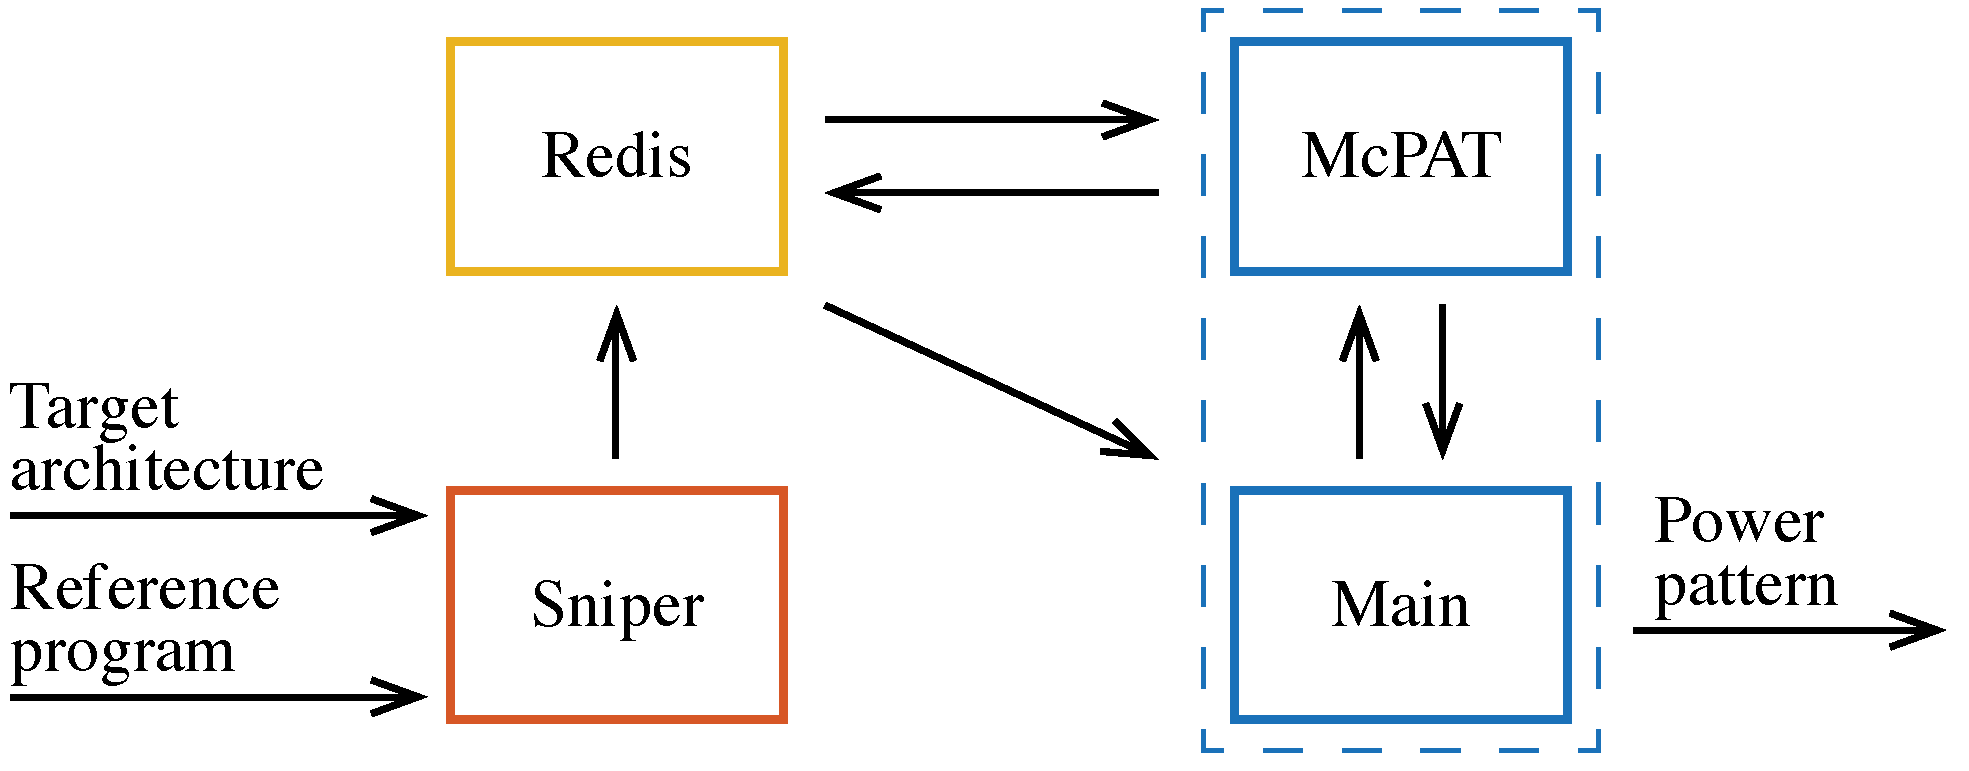
\includegraphics[width=1.0\columnwidth]{include/assets/figures/recorder.pdf}
  \caption{The recording infrastructure.}
  \flab{recorder}
\end{figure}

As the name suggests, the purpose of \recorder\ is recording. More specifically,
the tool records power traces, which are needed as an input to \streamer. The
recording infrastructure is depicted in \fref{recorder}.

Sniper \cite{carlson2011}.
\begin{table}
  \caption{Target architecture}
  \begin{tabular*}{\linewidth}{=L{70pt}l}
    \toprule
    Component    & Description \\
    \midrule
    Core         & 2660 MHz, 1.2 V \\
    L1-I/D cache & 32 KB, 4-way, LRU, private \\
    L2 cache     & 256 KB, 4-way, LRU, private \\
    L3 cache     & 8192 KB, 16-way, LRU, one per four cores \\
    \bottomrule
  \end{tabular*}
  \tlab{target}
\end{table}
% vim: nowrap tw=0


The key-value storage is Redis \cite{redis}. The database is SQLite
\cite{sqlite}.

\sc{McPAT} \cite{li2009}.


\subsection{Streamer} \slab{streamer}
\begin{figure}
  \centering
  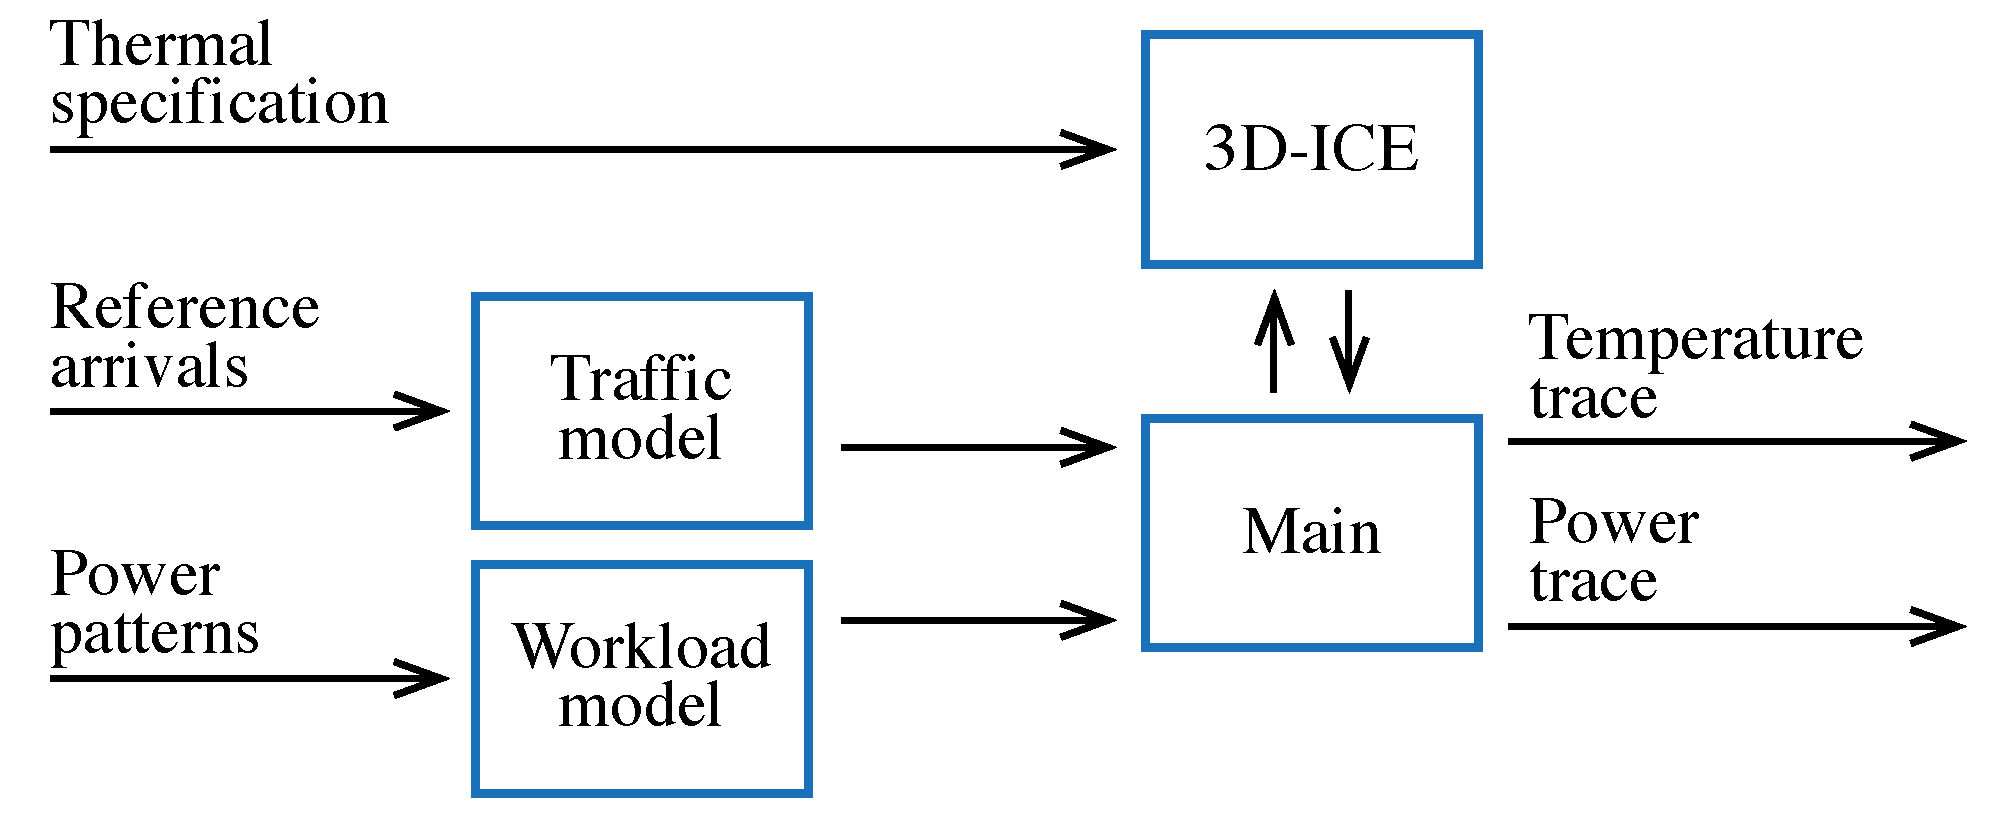
\includegraphics[width=1.0\columnwidth]{include/assets/figures/streamer.pdf}
  \caption{The streaming infrastructure.}
  \flab{streamer}
\end{figure}

The streaming infrastructure is depicted in \fref{streamer}.

HotSpot \cite{skadron2004}.
\sc{3D-ICE} \cite{sridhar2010}.
The solver is based on exponential integrators \cite{hochbruck2010},
\cite{ukhov2012}.


In the conclusion of this section, we would like to make a number of general
comments about the toolbox. First, as mentioned earlier, our tools are composed
of a number of packages, and we pursued a clear separation of the
responsibilities of these packages. As a result, the packages can be swapped out
or reused in other contexts. Second, we also provide auxiliary scripts and tools
(for instance, a tool for constructing die floorplans based on the information
from \sc{McPAT}), which are not elaborated on here but available as a part of
the toolchain. Last but not least, the toolbox is open source \cite{sources}.
